
\section{ Linear regresion }
\subsection{Stochastic gradient descendent}


Stochastic gradient descendent (SGD) is a sequential version of the gradient descent. Instead of considering the full batch gradient on all $N$
training data points, we condider a stochastic version of the gradient. Firts, pick a training data point $(x_n, y_n)$ uniformly random
(hence the name 'stochastic') and consider only the error on that data point.

The gradient of this single data point's error is used for the weight update in exactly the same that the gradient was used in batch gradient descent.


Motivo de 1, -1 para compensar la etiqueta

HAcer 200

W no importa en la práctica (podemos manipularlo)

VISUALIZAR MODELO CON SCATTER PLOT (DIAPOSITVA 22, CON LOS DATOS ENTRENAMIENTO Y TEST)t

E w deberá de ser la misma

Incluir valor de $E_in E_oit$ y eroro de clasificación (lo normal es que el error en test sea un poquito peor que los de entrenamiento.

Gradiente descendiente minimizar eterativamente:

En el segunto no tiene porqué darse que una iteración sea mejor (otra cosa es que mejore la tendencia mejor)

Si se utilizan todos sí que debería de ir mejorando de manera global.


\subsection{ How to plot }

As we know $w = ( cte, intensity-coeffinient, symmetry-coefficient) = (c,i,s)$ have three parameters. And we are going to plot in a 2D grap where

$c + x i + y s = 0$, it is a line, so we are going to compute two points, the one that x 

$(x = 0): y = frac{-c}{y}$
$(x=1): y = frac{-c - i}{y}$



\section{Experiment }

\subsection{a) Generate a training sample}

We are going to use a uniform generation:

\begin{minted}{python}
def simula_unif(N, d, size):
        ''' generate a trining sample of N  points
in the square [-size,size]x[-size,size]
'''
        return np.random.uniform(-size,size,(N,d))
 
\end{minted}

After fixed radom seed to $1$.

The final 2D map  is

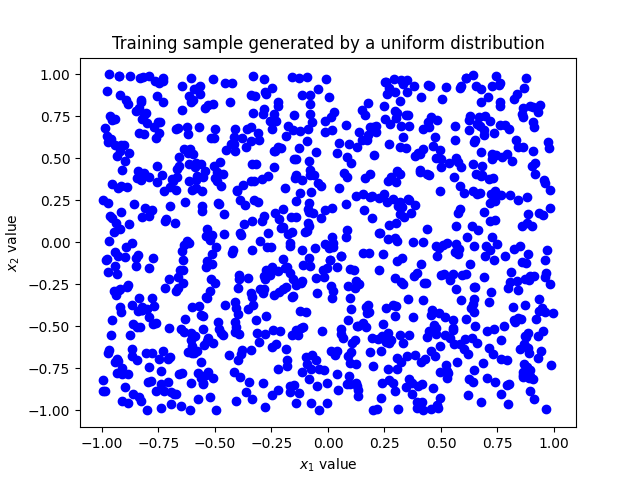
\includegraphics[width=\linewidth]{2_2_a_training_sample.png}

\subsection{b) Labels, noise and map}

b) Let's consider the function $f(x_1, x_2) = sign((x_1 - 0.2)^2 + x_2^2 - 0.6)$ that we will use to assign a label to each point of the previous sample. We introduce noise on the labels, randomly changing the sign of 10 \% of them.
Draw the obtained labels map.


Before plotting, while analysing the function is important to have in mind that a ciercumference with radius $r$ and center $(c_1, c_2) \in \mathbb R^2$ are the points $(x_1, x_2) \in \mathbb R^2$ that verify 

\[ (x_1 - c_1)^2 + (x_2 - c_2)^2 = r^2\]

Therefore looking at $f$ it is easy to think that we are goint to see a circle of radius $\sqrt{0.6}$ and center $(0.2, 0)$.

The plotting is

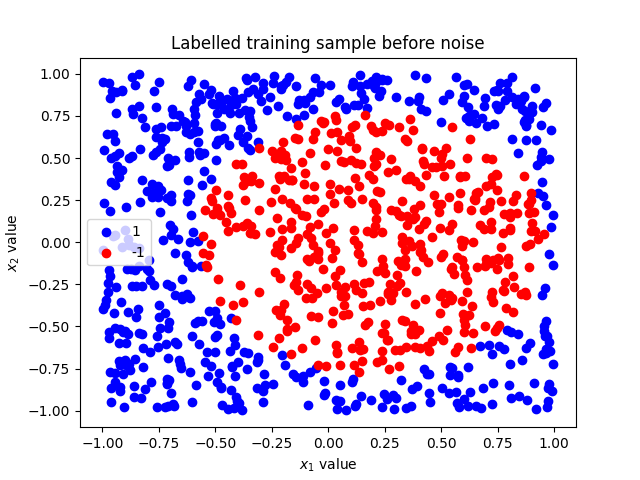
\includegraphics[width=\linewidth]{/2_2_b_labelled_before_noise.png}

In order to introduce noise on the label we are going to change randomly the sign of the $10\%$ of  the labels obtained by $b$.



\begin{minted}{python}
#labels 
y = np.array( [f(x[0],x[1]) for x in training_sample ])

index = list(range(size_training_example))
np.random.shuffle(index)

percent_noisy_data = 10.0
size_noisy_data = int((size_training_example *percent_noisy_data)/ 100 )


noisy_y = np.copy(y)
for i in index[:size_noisy_data]:
    noisy_y[i] *= -1

  \end{minted}

  As we can see the idea behind the snippet is simple: The noised labels would be a copy of the original one and $10\%$ of the data would change their sign.

  The final map is :


  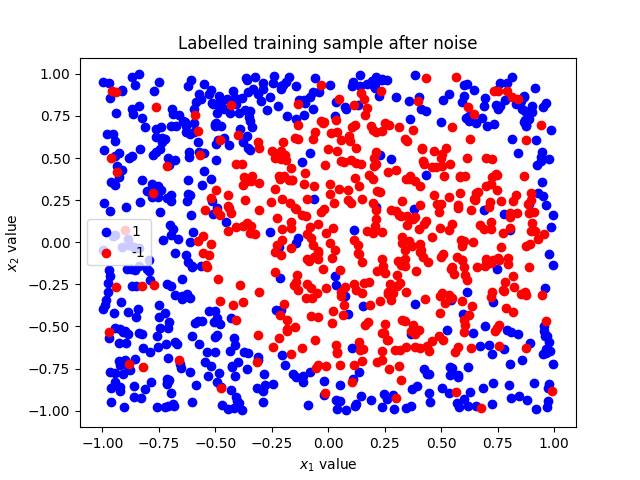
\includegraphics[width=\linewidth]{2_2_b_labelled_after_noise.png}
  

  \subsection{ Estimate the fitting error of $E_{in}$ using SDG}

  c) Using $(1, x_1, x_2)$ as feature vector, fit a linear regression model to the generated dataset and estimate the weights w. Estimate the fitting error of Ein using Stochastic Gradient Descent (SGD).

  Having in mind the observation in the last subsention that the labels follows a circumference equation with a bit of noise, a linear regression model it is not going to be the best approach.

  The experiment result are:
That for a linear SGD with batch size $32$ the $E_{in}$ is   $0.930$

And valuating output training data set
Input size:  1000
Bad negatives : 187
Bad positives : 224
Accuracy rate : 58.9 \%


Remember that the bad negatives are the points that the regression classify in negative but they are positives and the bad positives are the negatives one that are classify as a positives.

Finally the accuracy rate was the corrected classify data divided by the input size, so it is not a good model due to the fact that the accuracy rate is so close to a random one, that it would theoretically have a $50\%$ of a accuracy rate.

A visual representation of de fix is


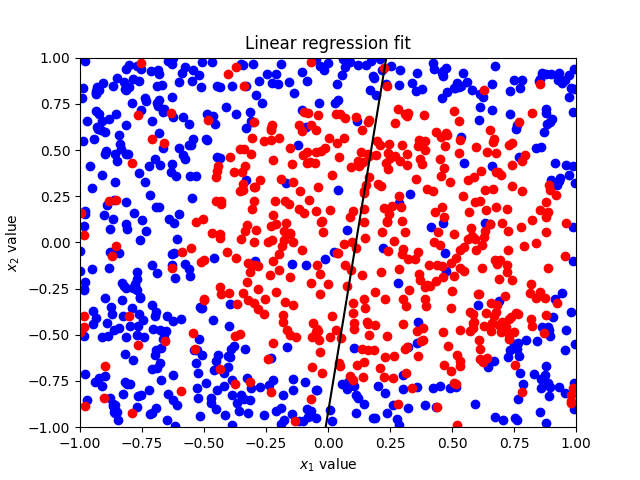
\includegraphics[width=\linewidth]{2_2_c_linear_regression.png}

